
\section{Spezielle sensorische Bahnen}
% verweis auf dieses Kapitel mit \ref{sec:spezsens}
\label{sec:spezsens}
Die speziellen sensorischen Bahnen umfassen unter anderem die Hörbahn \index{Hörbahn} und die Sehbahn\index{Sehbahn}, mit denen sich hauptsächlich dieses Kapitel beschäftigen wird. Es gibt weitere, spezialisierte Sinne, wie zum Beispiel den elektrischen Sinn bei Fischen, die beiden chemischen Sinne für Geruch und Geschmack und der Magnetsinn bei Zugvögeln \textsuperscript{\cite{smith2008biology}}. Diese werden nicht in dieser Zusammenfassung behandelt, spielen aber bei anderen Tierarten eine tragende Rolle und sollten aus diesem Grund hier kurz erwähnt werden.

\subsection{Hörbahn}

Das auditorische System \index{System! auditorisch} ist für die Verarbeitung von Schallwellen, die über die Luft oder Wasser übertragen und vom System empfangen werden, zuständig. Vibrationen, die über den Untergrund oder festes Substrat übertragen werden und mechanisch wahrgenommen werden, gehören zum Vibrationssinn, der eng mit dem auditorischen Sinn verwandt ist.
Dabei hat der auditorische Sinn zwei Aufgaben: Zum einen die Detektion des Schalls und zum anderen die Lokalisation der Schallwelle. Das Richtungshören ist jedoch nicht für alle Tiere möglich. Zudem ist es auch bei jenen Tieren, die dazu befähigt sind, nicht im gesamten Hörbereich gleich ausgelegt \textsuperscript{\cite[Kap.~18]{penzlin2005tierphys}}.

\subsubsection*{Cochlea und Hörnerv}
\index{Spiralganglion}
Die Funktion unserer Ohren ist die Energie eines akustischen Signals von der Außenwelt einzufangen und von einem mechanischen Signal in ein elektrisches umzuwandeln. Diese Umwandlung findet an den inneren Haarsinneszellen in der \textbf{Cochlea} statt. Dort wird durch die Auslenkung der Haarbündel an den  \textbf{inneren Haarsinneszellen} (eng.: inner hair cell, IHC) \index{Haarsinneszellen! innere, IHC} die Zelle depolarisiert oder hyperpolarisiert, je nach Auslenkungsrichtung \textsuperscript{\cite[Kap.~30]{kandel2013principles}}. Die Depolarisation der Haarzellen führt zur Öffnung spannungsgesteuerter Kalziumkanäle und dem damit verbundenen Einstrom von \ce{Ca^2+}. Durch den Einstrom des \ce{Ca^2+} wird der Neurotransmitter (wahrscheinlich Glutamat) freigesetzt und aktiviert die Spiralganglionzellen.  \textbf{Spiralganglionzellen} sind bipolare Zellen, welche ihren Namen der spiralförmigen Struktur der Cochlea ( \textbf{Schneckenspindel}) \index{Cochlea} verdanken, der sie folgen \textsuperscript{\cite[Kap.~11]{neurowissenschaften_baer}}. Sie formen einen Teil des achten Hirnnervs (CN~VIII), der auch  \textbf{Nervus vestibulocochlearis} \index{Hirnnerven! 08. N. vestibulocochlearis} genannt wird. Ungefähr 30~000  \textbf{Ganglionzellen} im Hörnerv werden durch die inneren Haarzellen erregt. Das macht ungefähr 90\% des Nervs aus \textsuperscript{\cite[Kap.~30]{kandel2013principles}}. 
Innere Haarzellen haben keinen efferenten Input von höheren Hirnstrukturen. Anhand der prozentualen Verteilung der verschiedenen Neuronentypen in der afferente Bahn wird die funktionale Bedeutung zwischen den inneren und äußeren Haarzellen deutlich. Die afferenten Fasern, ausgehend von den IHC, sind myelinisiert (Typ I) und bilden 95\% der afferenten Fasern, während 5\% der Fasern, afferente unmyelinsierte Typ~II Fasern, von den äußeren Haarzellen ausgehen. Bei den inneren Haarzellen gilt dabei die Regel, dass jedes Axon nur von einer Haarzelle erregt wird, eine Haarzelle erregt jedoch im Durchschnitt zehn Fasern.  \textsuperscript{\cite[Kap.~30]{kandel2013principles}}.   
\\
\noindent Die afferenten Nervenfasern der IHC kodieren die Stimulusfrequenz und dessen Intensität. Aufgrund der Beschaffenheit der Basilarmembran \index{Basilarmembran} der Cochlea, werden die Frequenzen tonotop von hohen Frequenzen am ovalen Fenster bis zu tiefen Tönen am Helicotrema \index{Helicotrema} entlang der Basilarmembran aufgeteilt \textsuperscript{\cite[Kap.~22]{paxinos2014rat}}. Infolge ihrer Größe und Funktion sind die Type I Fasern, ausgehend von den inneren Haarzellen, sehr viel besser verstanden. Die Bahnen, die die Informationen aus diesen Fasern führen, werden im Folgenden als einzige thematisiert.

\begin{figure}[H]
    \centering
    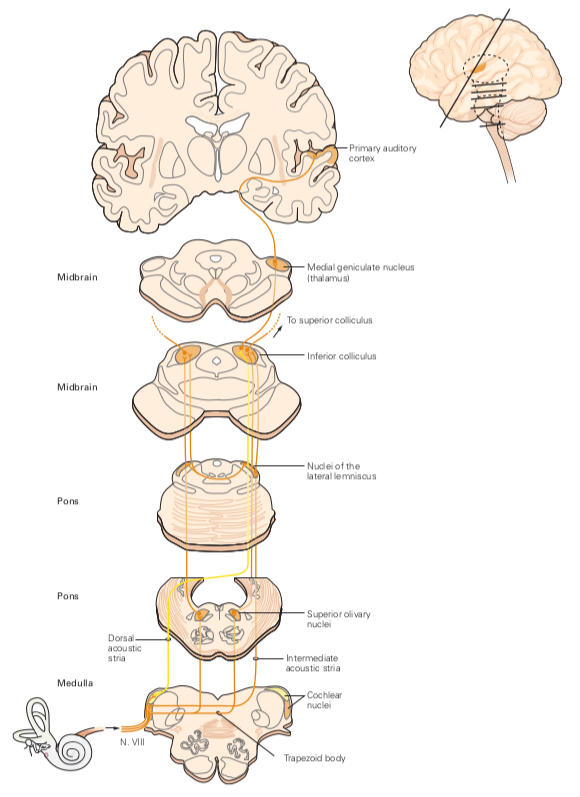
\includegraphics{pictures/auditory/hoerbahn_pathway.png}
    \caption[Hörbahn]{\textbf{Hörbahn.} Die einzelnen Stationen der Hörbahn des Menschen von den Spiralganglionzellen in der Cochlea bis zum primären auditorischen Cortex anhand skizzierter Gehirnschnitte. Abbildung nach \textit{Principles of Neural Science}, Kandel et al. \textsuperscript{\cite[Kap.~30]{kandel2013principles}}.}
    \label{fig:hoerbahn_pathway}
\end{figure}

\newpage
\noindent Efferente Fasern im Hörnerv innervieren die äußeren Haarzellen \index{Haarsinneszellen! äußere, OHC} in der Cochlea, deren Aufgabe darin besteht die mechanische Auslenkung der Basilarmembran und der damit verbundenen Tektorialmembran \index{Tektorialmembran} zu verstärken oder zu unterdrücken. Infolgedessen kommt es zu einer verstärkten Selektivität und Sensibilität der Frequenzwahrnehmung \textsuperscript{\cite[Kap.~22]{paxinos2014rat}}.

\subsubsection*{Nucleus cochlearis}

Die afferenten Ganglionzellen aus dem Hörnerv ziehen auf der Höhe der Medulla in den Hirnstamm und dort in das Kerngebiet des \textbf{Nucleus cochlearis} (CN). \index{Nucleus! cochlearis} Dieser befindet sich  lateral auf Höhe der  \textbf{Medulla} (Abb.~\ref{fig:hoerbahn_pathway}) und bekommt nur Input aus dem Hörnerv der ipsilateralen Seite. Der CN besteht aus dem  \textbf{dorsalen Nucleus cochlearis} (DCN) und dem  \textbf{ventralen Nucleus cochlearis} (VCN), welcher wiederum in den anteroventralen (AVCN) und den posteroventralen (PVCN) Nucleus unterteilt wird \textsuperscript{\cite[Kap.~22]{paxinos2014rat}}. Bei Ratten liegt der ventrale Nucleus cochlearis mediolateral flach an der Medulla, während der dorsale Nucleus cochlearis sich um den unteren Kleinhirnstiel (engl.: restiform body) \textsuperscript{\cite[Kap.~22]{paxinos2014rat}} zieht.

\begin{figure}[H]
    \centering
    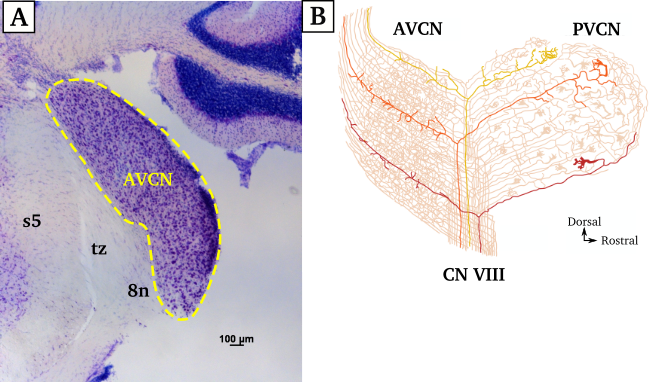
\includegraphics[width = \textwidth]{pictures/auditory/CN.png}
    \caption[Nucleus cochlearis]{\textbf{Nucleus cochlearis.} \textbf{A:} Nissl-Färbung (N09-1) der rechten Seite der Medulla. Es sind der anteroventrale Nucleus cochlearis (AVCN), der Trigeminus (s5), der Trapezkörper (tz) und der achte Hirnnerv (8n, Hörnerv) zu sehen. \textbf{B:} Verlauf der Nervenfasern aus dem achten Hirnnerv (CN VIII, 8n) im ventralen Nucleus cochlearis. Sowohl im anteroventralen (AVCN) als auch im posteroventralen (PVCN) Bereich des CNs werden die Fasern nach der Frequenz tonotop geordnet, von den tiefen Frequenzen (rot) ventral bis zu den hohen Frequenzen (gelb) im dorsalen Bereich. \\
    Abbildung B nach \textit{Principles of Neural Science}, Kandel et al. \textsuperscript{\cite[Kap.~31]{kandel2013principles}}, abgeändert.}
    \label{fig:Nucleus_cochlearis}
\end{figure}


\noindent Die auditorischen Nervenfasern verzweigen sich im Nucleus cochlearis in die verschiedenen Teile des CNs (Abb.~\ref{fig:Nucleus_cochlearis}~B). Jede Faser gabelt sich in einen aufsteigen Ast zum AVCN und einen absteigenden Ast zum PVCN und DCN und leitet die Informationen an verschiedene Neurone dieser Teilbereiche weiter \textsuperscript{\cite[Kap.~22]{paxinos2014rat}}. Die Neurone im ventralen Nucleus cochlearis kodieren für verschiedene Eigenschaften, je nach Zelltyp. Im Allgemeinen schärfen sie das Timing und die Informationen aus dem Klangspektrum. 

\noindent Eine wesentliche Rolle spielt die Interauralezeitdifferenz bei der Weiterverarbeitung der Informationen in der  \textbf{oberen Olive}, wohingegen die Verarbeitung des Klangspektrums in den ipsilateralen DCN, die ipsilaterale laterale obere Olive (LSO), den contralateralen ventralen Nucleus des lateralen Lemniscus und den contraleteralen Colliculus inferior projiziert wird \textsuperscript{\cite[Kap.~31]{kandel2013principles}}. 

\noindent Der dorsale Nucleus cochlearis bekommt einerseits direkten Input von den Neuronen aus dem Hörnerv, zum anderen indirekten Input aus dem ventralen CN. Der dorsale CN integriert akustische und somatosensorische Informationen um die Richtung der Schallquelle zu bestimmen \textsuperscript{\cite[Kap.~31]{kandel2013principles}}. 


\subsubsection*{Obere Olive}
\index{Olive! obere Olive}
Ein Großteil der Nervenzellen aus dem Nucleus cochlearis projizieren in die obere Olive. Die \textbf{obere Olive} (\textit{Nucleus olivaris superior}) ist für die Verarbeitung auditorischer Informationen wichtig und umfasst mehrere Kerngebiete. Innerhalb der Säugetiere variieren diese Kerngebiete. Drei Kerngebiete können bei fast allen Spezies gefunden werden: Die \textbf{laterale obere Olive} (engl.: lateral superior olive, \textbf{LSO}), die \textbf{mediale obere Olive} (engl.: medial superior olive, \textbf{MSO}) und der \textbf{mediale Nucleus des Trapezkörpers} (engl.: medial nucleus of the trapezoid body, \textbf{MNTB}). Die LSO ist ein S-förmiges Kerngebiet im lateralen Bereich der oberen Olive. Sie ist durch ihre markante Struktur leicht zu erkennen (Abb.~\ref{fig:obere_Olive}). Die MSO liegt medial der LSO und ist bei Ratten ein deutlich kleineres Kerngebiet als beim Menschen. Der mediale Nucleus des Trapezkörpers (MNTB) befindet sich lateral in der oberen Olive \textsuperscript{\cite[Kap.~29]{paxinos2014rat}}.

In Nagetieren, wie der Ratte, gibt es ein viertes, ausgeprägtes Kerngebiet, den \textbf{oberen paraoliven Nucleus} (engl.: superior paraolivary nucleus, \textbf{SPO}). Dieses Kerngebiet befindet sich im dorsomedialen Bereich der oberen Olive. Es bekommt Informationen aus dem contralateralen Nucleus cochlearis und projiziert in den Colliculus inferior auf der ipsilateralen Seite \textsuperscript{\cite[Kap.~29]{paxinos2014rat}}. Die SPO entschlüsselt besonders gut Muster in Tönen, sowie Informationen in zeitlichen Mustern. Das spielt in der Wahrnehmung von Kommunikation eine wichtige Rolle, im Besonderen bei akustischen Schwebungen in Vokalisationen bei Tieren und Sprachsignalen beim Menschen \textsuperscript{\cite[Kap.~29]{paxinos2014rat}}. 
\\

\noindent Die drei Hauptkerne der oberen Olive spielen eine wichtige Rolle in der Verarbeitung von Schall. Aufgrund der Beschaffenheit der Cochlea werden dort nur die einzelnen Frequenzen kodiert. Es werden keine Informationen über die Richtung der Schallquelle kodiert. Das Richtungshören wird in der oberen Olive, durch die Verarbeitung der Informationen aus beiden Ohren, integriert. Sie ist damit die erste Schaltstelle in der Hörbahn, die Input sowohl von der ipsilateralen, als auch von der contralateralen Seite, aus den jeweiligen Nuclei cochlearis, bekommt.
\\

\index{Olive! obere Olive! MSO}
\noindent Die \textbf{mediale obere Olive} (\textbf{MSO}) ist tonotop arrangiert. Die tiefen Töne werden dorsal in der MSO verarbeitet, wohingegen hohe Frequenzen im ventralen Part verarbeitet werden. Der Anteil der tiefen Töne ist in der MSO proportional über repräsentiert. Aus diesem Grund ist die MSO in der Ratte (Abb.~\ref{fig:obere_Olive}) klein, da Ratten im hochfrequenten Bereich hören.

Die mediale obere Olive erhält exzitatorischen Input aus den beiden Nuclei, wobei die lateralen Dendriten der MSO, die Informationen aus dem ipsilateralen Nucleus cochlearis erhalten und die medialen Dendriten aus dem contralateralen Nucleus \textsuperscript{\cite[Kap.~29]{paxinos2014rat}}. Da die Neurone aus den Nuclei nur zu einer bestimmt Phase des Tons feuern (engl.: \textbf{phase-locking}), kann mit Hilfe der interauralen Zeitdifferenz und dem 'coincidence detection model' die Richtung, aus der der Ton kam, bestimmt werden \textsuperscript{\cite[Kap.~31]{kandel2013principles}}. Da der interaurale Abstand bei Ratten sehr klein ist, ist die Zeitdifferenz zwischen den Ohren ebenfalls sehr klein. Er lässt sich nur für sehr tiefe Töne berechnen.

Die Axone der MSO projizieren in den \textbf{dorsalen Nucleus des lateralen Lemniscus} (\textbf{DLL}) und in den \textbf{Colliculus inferior} (\textbf{IC}) \textsuperscript{\cite[Kap.~29]{paxinos2014rat}}.
\\

\begin{figure}[H]
    \centering
    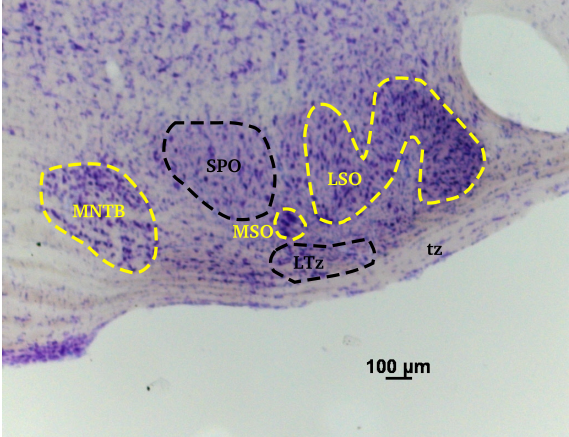
\includegraphics{pictures/auditory/obere_olive.png}
    \caption[Obere Olive]{\textbf{Obere Olive.} Nissl-Färbung (N10-1) der oberen Olive des Pons. Mit den drei Hauptkernen: Der mediale obere Olive (MSO), der lateralen oberen Olive (LSO) und dem medialen Nucleus des Trapezkörpers (MNTB), sowie dem für Nager speziellen oberen paraoliven Nucleus (SPO). Des Weiteren liegen in der oberen Olive das Kerngebiet des lateralen Nucleus des Trapezkörpers (LTz) und der Trapezkörper (tz) selbst. Letzterer verbindet die oberen Oliven beider Hemisphären miteinander und befindet sich ventral des Komplex der oberen Olive.}
    \label{fig:obere_Olive}
\end{figure}

Die \textbf{laterale obere Olive} (\textbf{LSO}) und der \textbf{mediale Nucleus des Trapezkörpers} (\textbf{MNTB}) \index{Nucleus! MNTB} bilden gemeinsam eine Einheit, welche über die Berechnung der interauralen Intensitätsdifferenz das Richtungshören bei hohen Tönen ermöglicht. 
Die tonotop Anordnung der LSO zieht sich entlang der S-Form von hohen Tönen (medial) bis zu tieferen Tönen (lateral). Die LSO der Ratte ist im Vergleich zum Menschen deutlich größer. Das hängt unter anderem mit der Überrepresentation der hohen Töne in der lateralen oberen Olive und dem Hörbereich von Ratten zusammen.

Die LSO erhält bilateralen Input. Der ventrale Nucleus cochlearis (VCN) der ipsilateralen Seite leitet die Informationen exzitatorisch an die LSO weiter. Vom contralateralen VCN werden die Informationen exzitatorisch an den MNTB, der jeweils anderen Seite, über den Trapezkörper weiter gegeben. Von dort aus wird das Signal inhibitorisch an die LSO derselben Seite weiter geleitet.
Somit bekommen die Neurone der LSO indirekten inhibitorischen Input aus dem contralateralen Nucleus cochlearis und exzitatorischen Input aus dem ipsilateralen Nucleus cochlearis.

Die laterale obere Olive projiziert bilateral in den zentralen Nucleus des  \textbf{Colliculus inferior} (\textbf{IC})\index{Colliculus! inferior}. Es wird auf die ipsilaterale Seite inhibitorisch, auf die contralaterale Seite exzitatorisch projiziert.
Des Weiteren projiziert ein Teil der Neurone auch in den dorsalen Nucleus des lateralen Lemniscus (\textbf{DLL}) \textsuperscript{\cite[Kap.~29]{paxinos2014rat}}.


\subsubsection*{Lateraler Lemniscus}
\index{Lemniscus! lateral}
Die afferenten Nervenfasern aus der oberen Olive bilden den \textbf{Lemniscus lateralis} (\textbf{ll}), welcher über das Tegmentum pontis in den \textbf{Colliculus inferior} (\textbf{IC}) \index{Colliculus! inferior} zieht und dort terminiert (Abb.~\ref{fig:lateraler_lemniscus}). Einige der Axone aus der oberen Olive terminieren in den \textbf{Nuclei des lateralen Lemniscus}. Des Weiteren enden hier auch Nervenfasern, die direkt aus den Nuclei cochlearis kommen \textsuperscript{\cite[Kap.~10]{crossman2014neuroanatomy}}. 
Die Nuclei des lateralen Lemniscus unterteilen sich in den \textbf{dorsalen Nucleus des lateralen Lemniscus} (\textbf{DLL}) \index{Nucleus! dorsaler Nucleus des lateralen Lemniscus} und den \textbf{ventralen Nucleus des lateralen Lemniscus} (\textbf{VLL}). \index{Nucleus! ventraler Nucleus des lateralen Lemniscus} Diese Unterteilung erfolgt anhand zweier funktional unterschiedlichen Systeme: die monoaurale Verarbeitung ventral und die binaurale Verarbeitung dorsal \textsuperscript{\cite[Kap.~29]{paxinos2014rat}}. 
\\

Afferente Neurone ziehen aus dem contralateralen ventralen Nucleus cochlearis (VCN) und dem ipsilateralen MNTB in den \textbf{ventralen Nucleus des lateralen Lemniscus} (\textbf{VLL}). Der VLL ist vorwiegend für die Verarbeitung von präzisen zeitlichen Informationen zuständig.
Es wird vermutet, dass die Zwischenstation in dem ventralen Nucleus als Relaisstation auf dem Weg zum Colliculus inferior fungiert.
Der Nucleus ist aus isofrequenten Lamina aufgebaut und liegt im Pons (Abb.~\ref{fig:lateraler_lemniscus}). Die Afferenzen zum Colliculus inferior sind ebenfalls tonotop arrangiert. Sie terminieren im zentralen Bereich des IC \textsuperscript{\cite[Kap.~29]{paxinos2014rat}}.
\\

Der \textbf{dorsale Nucleus des lateralen Lemniscus} (\textbf{DLL}) liegt oberhalb des ventralen Nucleus des lateralen Lemniscus im Pons (Abb.~\ref{fig:lateraler_lemniscus}). Er bekommt bilateralen Input. Diesen bekommt er von der contralateralen Seite aus dem ventralen Nucleus cochlearis (VCN) und dem DLL. Von der ipsilateralen Seite projizieren afferente Nervenfasern aus der MSO, SPO und dem VLL in den DLL. Zudem ziehen aus beiden Seiten Afferenzen aus der lateralen oberen Olive (LSO) in den DLL.
Aufgrund der vielen Verbindungen zu tiefer liegenden Kernen, wie der LSO und MSO, spielt der dorsale Nucleus eine wichtige Rolle beim Richtungshören. Läsionen im DLL bewirken ein Defizit im Richtungshören und eine Ungenauigkeit in der räumlichen Hörschärfe. 
Der DLL projiziert über den lateralen Lemniscus in beide Colliculi inferiores (IC) und über die Probst Kommissur in den gegenüberliegenden dorsalen Nucleus des lateralen Lemniscus
\textsuperscript{\cite[Kap.~29]{paxinos2014rat}}.

\begin{figure}[H]
    \centering
    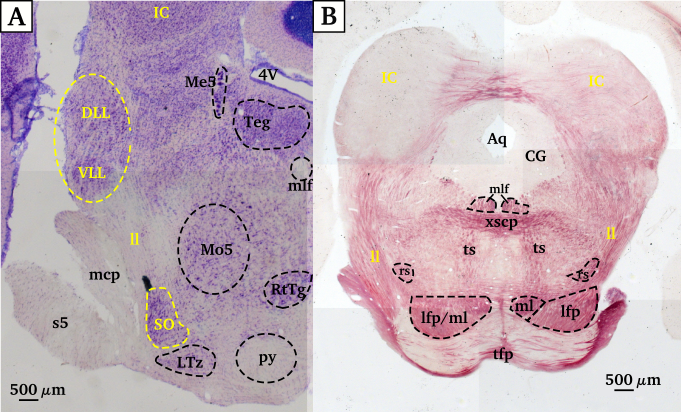
\includegraphics[width = \textwidth]{pictures/auditory/lateral_lemniscus.png}
    \caption[Der Lateraler Lemniscus und seine Kerne]{\textbf{Der Lateraler Lemniscus und seine Kerne.} Verlauf des lateralen Lemniscus und die Lage seiner Kerne in der Nissl-Färbung (N11-4) und der Faser-Färbung (F13-4). Die Schnittebenen sind 1200~$\upmu$m auseinander.\\
    \textbf{A:} Nissl-Färbung (N11-4) auf der Höhe des Pons, erkennbar am vierten Ventrikel (4V).
    Der laterale Lemniscus verbindet die obere Olive (SO) mit dem Colliculus inferior (IC). Einige der Verbindungen sind über den dorsalen (DLL) oder den ventralen (VLL) Nucleus des lateralen Lemniscus zwischen geschaltet. 
    Des Weiteren sind der Trigeminus (s5) und der Nucleus des mesencephalischen Trakts des Trigeminus (Me5) aus der Somatosensorik, sowie der motorische Nucleus des Trigeminus (Mo5) aus der Motorik zu sehen. 
    Weitere Kerngebiete und Fasertrakte sind: lateraler Nucleus des Trapezkörpers (LTz), mittleres cerebellare Pendunkel (mcp), medialer Fasciculus longitudinalis (mlf), Pyramidenbahn (py), reticulotegmentaler Nucleus des Pons (RtTg), Tegmentum (Teg).\\
    \textbf{B:} Verlauf des lateralen Lemniscus (ll) bis in den Colliculus inferior (IC) im Mesencephalon. Das zentrale Höhlengrau (CG) und das Aquädukt (Aq) sind zwei prominente Strukturen, die im Mesencephalon liegen. Des Weiteren sind folgende Fasertrakte zu sehen: Fasciculus longitudinalis des Pons (lfp), medialer Lemniscus (ml), medialer Fasciculus longitudinalis (mlf), rubrospinaler Trakt (rs), transversale Fasern des Pons (tfp), tectospinaler Trakt (ts), Kreuzung (Dekussation) des oberen cerebellaren Pedunkels (xscp).}
    \label{fig:lateraler_lemniscus}
\end{figure}

\newpage
\subsubsection*{Colliculus inferior und Corpus geniculatum mediale}

Die Fasern des lateralen Lemniscus ziehen in den \textbf{Colliculus inferior} (\textbf{IC}) \index{Colliculus! inferior} und terminieren dort. Der IC liegt bei der Ratte sichtbar im dorsalen Bereich des Mittelhirns, caudal vom Colliculus superior, mit dem er gemeinsam die Vierhügelplatte bildet (Kap.~\ref{subsubsec:Tectum}) \textsuperscript{\cite[Kap.~29]{paxinos2014rat}}. 
Der IC integriert nahezu die gesamt Information aus den tiefer liegenden auditorischen Kerngebieten des Hirnstamms. Das macht ihn zu einem großen Integrationszentrum für die Verarbeitung des Richtungshörens, sowie für Tonhöhen \textsuperscript{\cite[Kap.~29]{paxinos2014rat}}.

\begin{figure}[H]
    \centering
    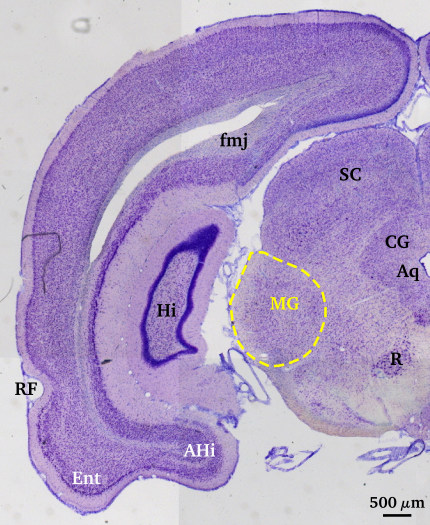
\includegraphics{pictures/auditory/MG.png}
    \caption[Corpus geniculatum mediale]{\textbf{Corpus geniculatum mediale.} Das Corpus geniculatum mediale (MGN) liegt im Mesencephalon lateral-ventral des Colliculus superior (SC). Das Aquädukt (Aq) wird vom zentralen Höhlengrau (CG) umgeben und unterhalb liegt der Nucleus ruber (R), welcher sich ebenfalls im Mesencephalon befindet. Der Cortex liegt um das Mesencephalon herum. Dazu zählen der amygdaloid-hippocampale Bereich (AHi) der Cortex entorhinalis (Ent), Forceps major des Corpus callosum (fmj) und der Hippocampus (Hi). Nissl-Färbung (N16-3)}
    \label{fig:MG}
\end{figure}

Vom Colliculus inferior aus zieht die Hörbahn in den \textbf{medialen Kniehöcker} (\textit{Corpus geniculatum mediale}). \index{Corpus! geniculatum mediale} Der mediale Kniehöcker (\textbf{MGN}) liegt auf der posterolateralen Seite des Thalamus (Abb.~\ref{fig:MG}). Er ist eine runde Erhebung lateral-ventral des Colliculus superior. Der MGN ist das letzte Integrationszentrum in der auditorischen Hörbahn vor dem Cortex. Er bekommt Input aus dem Colliculus inferior (IC) über das \textit{Brachium colliculi inferioris}. Zudem terminieren absteigende Fasern aus dem auditorischen Cortex und dem reticularen Nucleus im MGN. Afferente Nervenfasern aus dem medialen Kniehöcker ziehen ipsilateral in den auditorischen Cortex \textsuperscript{\cite[Kap.~29]{paxinos2014rat}}. Der mediale Kniehöcker ist in drei Untereinheiten aufgeteilt: den ventralen, den dorsalen und den medialen Part. Der ventrale mediale Kniehöcker hat eine rein akustische Funktion, wohingegen der dorsale Part bei akustischer Aufmerksamkeit mitwirkt und der mediale Part bei multisensorischer Erregung und emotionalem akustischen Lernen eine Rolle spielt \textsuperscript{\cite[Kap.~29]{paxinos2014rat}}. 
\\
Eine weitere Bahn führt vom Colliculus inferior direkt in den Colliculus superior (SC), welcher bei reflexiven Bewegungen zur Orientierung eine Rolle spielt. Deswegen wird angenommen, dass im SC eine auditorische Karte der Umgebung erstellt wird. Ein Beispiel dafür sind Eulen, bei denen man solche zwei-dimensionalen Karten gefunden hat. Zusammen mit Karten aus dem visuellen System und dem somatosensorischen System spielt der Colliculus superior \index{Colliculus! superior}eine entscheidende Rolle in der motorischen Orientierung während dem Greifen nach Gegenständen \textsuperscript{\cite[Kap.~31]{kandel2013principles}}.


\subsubsection*{Primärer auditorischer Cortex}
\index{Cortex! primär auditorisch}

Die Fasern aus dem medialen Kniehöcker enden in einer tonotopen Anordnung, tiefe Frequenzen werden anterolateral und hohe Frequenzen posteromedial in der primären Hörrinde beim Menschen repräsentiert \textsuperscript{\cite[Kap.~9.9]{trepel2011neuroanatomie}}. Die Fasern aus der Hörbahn enden in den Heschl-Querwindungen des Temporallappens. Der primäre auditorische Cortex (Brodmann's Areal 41 und 42) liegt im Temporallappen, genauer gesagt im oberen Gyrus des Temporallappens, versteckt im \textit{Sulcus lateralis} \index{Sulcus! lateralis} \textsuperscript{\cite[Kap.~13]{crossman2014neuroanatomy}}. 

Die primäre Hörrinde, auch \textbf{primärer auditorischer Cortex} (\textbf{A1}) genannt, erhält akustische Informationen aus der bisher beschriebenen Hörbahn. Aufgrund der Verschaltung der Hörbahn bekommt sowohl die linke, als auch die rechte Großhirnhemisphäre, sowie das dort liegende primäre auditorische Areal, Informationen aus beiden Ohren. Einige Eigenschaften, wie die interaurale Zeitdifferenz und die interaurale Intensitätsdifferenz, die in der oberen Olive berechnet werden, werden hier zum entgültigen Richtungshören integriert. 

Die primären Hörrinde ist für das interpretationsfreie bewusst werden von wahrgenommenen auditorischen Signalen veranwortlich. Das heißt im Klaren, wenn man im primären auditorischen Cortex reizt, werden Laute und Muster wahrgenommen, aber keine Melodien oder Sprache. Die Zusammensetzung einzelner Laute zu Srache geschieht erst in der sekundären Hörrinde \textsuperscript{\cite[Kap.~9.9]{trepel2011neuroanatomie}}.

\subsubsection*{Sekundärer auditorischer Cortex und cortico-cortikale Verbindungen}

Der \textbf{sekundäre auditorische Cortex} \index{Cortex! sekundär auditorisch} liegt lateral der primären Hörrinde und nimmt die Brodmann Areale 42 und 22 ein. Der Cortex erhält Input aus der primären Hörrinde. Dabei ist die Verarbeitung auf beiden Hemisphären unterschiedlich. Bei Rechtshändern wird auf der linken Großhirnhälfte der sekundäre auditorische Cortex auch \textbf{Wernicke-Areal} \index{Wernicke-Areal} genannt. Das Wernicke-Areal (Abb.~\ref{fig:Wernicke}) integriert die auditorischen Informationen für das Verständnis von Sprache. Der sekundäre auditorische Cortex integriert die auditorischen Informationen auf eine mehr rationale Art. Die Hemisphäre auf der die Sprache verarbeitet wird, ist die dominante Hemisphäre. Dies steht im Gegensatz zur Verarbeitung des sekundären auditorischen Cortex auf der rechten Hemisphäre bei Rechtshändern. Dort werden mehr 'nicht-rationale' Komponenten verarbeitet. Dazu zählt das Erkennen und Verständnis von Musik. Man nennt diese Hemisphäre auch die nicht-dominante Hemisphäre. Für Rechtshänder trifft die oben genannte Einteilung in dominante Hemisphäre links und nicht-dominante Hemisphäre rechts zu. Für Linkshänder ist die Einteilung weniger klar: Die nicht-dominante Hemisphäre kann rechts oder links sein \textsuperscript{\cite{trepel2011neuroanatomie}}.

Weiteren Input bekommt der sekundäre auditorische Cortex vom \textbf{Gyrus angularis}, welcher wiederum mit dem sekundären visuellen Cortex verknüpft ist. Diese Verbindung spielt eine Rolle beim Verständnis von gelesener Sprache. Die gesehene Schrift oder das Benennen von gesehenen Gegenständen wird im Wernicke-Areal mit dem Sprachverständnis verknüpft. 

Das Wernicke-Areal ist über den \textbf{Fasciculus arcuatus} \index{Fasciculus! arcuatus} mit dem \textbf{Broca-Areal} \index{Broca-Areal} verknüpft. Das Broca-Areal (Brodmanm Areal 44 und 45) liegt im Frontallappen und gehört zum Motorcortex. Dieses Konstrukt wird \textbf{Wernicke-Gerschwind Modell} \index{Wernicke-Gerschwind Modell} genannt und verbindet das Sprachverständnis im Wernicke-Areal mit der Sprachproduktion im Broca-Areal. Einige Zeit nahm man an, dass diese Verbindung (Fasciculus arcuatus) nur unidirektional ist. Studien belegten aber, dass der Informationsfluss in beide Richtungen läuft und auch noch weitere Gehirnareale an dem Verständnis und der Produktion von Sprache beteiligt sind \textsuperscript{\cite[Kap.~60]{kandel2013principles}}.

\begin{figure}[H]
    \centering
    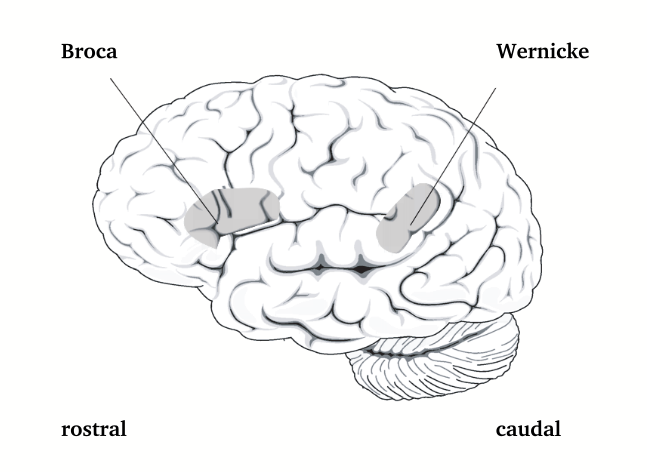
\includegraphics[width=0.8\textwidth]{pictures/auditory/Wernicke.png}
    \caption[Wernicke-Areal]{\textbf{Wernicke-Areal.} Wernicke-Areal und Broca-Areal auf der dominanten (linken) Hemisphäre. Die Verbindung der Beiden Areale (Fasciculus arcuatus) ist nicht abgebildet, verläuft aber um den Sulcus lateralis herum.\\
    Abbildung verändert, nach \url{https://www.nidcd.nih.gov/health/aphasia}.}
    \label{fig:Wernicke}
\end{figure}

\newpage
\subsection{Sehbahn}

Die \textbf{Sehbahn} ist die Bahn in welcher die Verarbeitung der eingehenden Informationen aus den Lichtsinneszellen in der Retina erfolgt. Die visuelle Wahrnehmung ist für den sehenden Menschen eine kaum wegzudenkende Informationsquelle ihrer Umgebung. Das Leben des Menschen ist zum Großteil darauf ausgerichtet, dass dieser sehen kann. Unter anderem nehmen wir auf diese Weise die Gefühlsregungen unserer Mitmenschen wahr, da diese über den Gesichtsausdruck ihr Empfinden ausdrücken. Wir Menschen verlassen uns außerdem noch auf das Sehen für die Orientierung, Objekterkennung und abstrakteres Erleben, wie zum Beispiel Kunst, Erinnerungen und Lesen.


\subsubsection*{Das Auge}
\index{Auge}
Das Auge ist das primäre Sehsinnesorgan. Dort befinden sich die lichtbrechenden Strukturen, wie die \textbf{Cornea} \index{Cornea} und die \textbf{Linse} \index{Linse}. Diese Strukturen  bestimmen die Abbildungsqualität auf der Retina. Die \textbf{Retina} ist die Zellstruktur in der die Lichtimpulse durch die \textbf{Photorezeptoren} wahrgenommen werden. Das Signal wird über die \textbf{Bipolarzellen} zu den \textbf{Ganglionzellen} weitergeleitet, welche dann wiederum die Informationen bis ins Gehirn weitergeben.
Das Auge der Säugetiere ist ein invertes Linsenauge, \index{Linsenauge} das sich zu Teilen aus dem Diencephalon entwickelt. 
\\
\\
Das Auge der Säugetiere ist eine Struktur, die sich im Laufe der embryonalen Entwicklung aus Zellen des Ektoderms und des Mesoderms entwickeln. Bei der Entwicklung der Neurula differenzieren Zellen im dorsalen Bereich zu Neuroektodermzellen \index{Neuroektoderm} (Abb.~\ref{fig:eye_neurulation}~A). Diese entwickeln sich im weiteren Verlauf zur Neuralplatte und dann zum Neuralrohr (Kap.~\ref{subsec:Neurulation}). 
Es wird angenommen, dass in einem frühen Stadium der evolutionären Entwicklung, als unserer Vorfahren noch freischwimmende Lebewesen waren, deren ursprüngliche Photorezeptoren in einem 'Streifen reaktiver Zellen' lagen. Diese waren nach außen gerichtet, ähnlich des Aufbaus des Linsenauges bei Weichtieren. Bei den heutigen Säugetieren liegen die Photorezeptoren, aufgrund der Einstülpung des Ektoderms während der Neurulation, dann abgewandt vom Licht auf der Innenseite des Auges. 

Bei der Entwicklung des Embryos, nach der Einstülpung zum Neuralrohr, entwickeln sich dann die Gehirnbläschen oder Gehirnventikel (Abb.~\ref{fig:eye_neurulation}~C). Aus dem Diencephalon stülpt sich ein Teil des Ektoderms aus und entwickelt sich zum optischen Ventrikel (Abb.~\ref{fig:eye_neurulation}~D), welches sich dann zur \textbf{Augengrube} \index{Augengrube} entwickelt. Aus dieser wiederum entsteht dann die Retina. Die Linse das Auges entwickelt sich währenddessen ebenfalls aus ektodermalen Zellen. Diese Entwicklung wird durch die Zellen des \textbf{optischen Ventrikel} \index{optischer Ventrikel} im Mesoderm induziert. Es entsteht eine sogenannte \textbf{Linsenplakode} \index{Linsenplakode} (Abb.~\ref{fig:eye_neurulation}~E), welcher sich einstülpt und dann abspaltet (Abb.~\ref{fig:eye_neurulation}~F~\&~G). Der Rest des Auges entwickelt sich aus dem Mesoderm \textsuperscript{\cite[Kap.~16]{smith2008biology}}.

\begin{figure}[H]
    \centering
    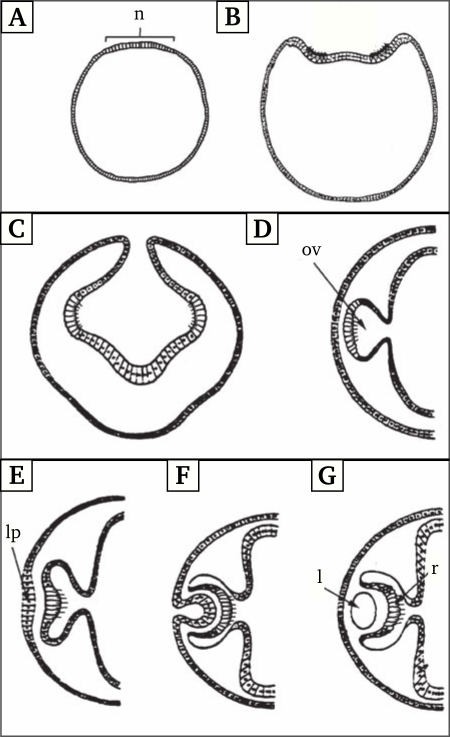
\includegraphics{pictures/visual/Eye_Neurulation.png}
    \caption[Embryonale Entwicklung des Auges]{\textbf{Embryonale Entwicklung des Auges.} \textbf{A:} Neurula mit Neuroektodermzellen (n). \textbf{B:} Blastula mit ausgebildeter Neuralplatte. \textbf{C:} Einstülpung zum Neuralrohr. \textbf{D:} Entwicklung des optischen Ventrikels (ov) aus dem Diencephalon. \textbf{E:} Migration der Ektodermzellen ins Mesoderm für die Bildung der Linse (Linsenplakode, lp). \textbf{F:} Bildung der Augengrube und Einstülpung der Linsenplakode. \textbf{G:} Linse (l) und Photorezeptoren (r) auf der abgewandten Seite des Lichts.\\
    Abbildung nach \textit{Biology of Sensory Systems}, Smith \textsuperscript{\cite[Kap.~16]{smith2008biology}}.}
    \label{fig:eye_neurulation}
\end{figure}


\subsubsection*{Die Retina}

\index{Retina}

Die Retina ist in laminaren Schichten aufgebaut (Abb.~\ref{fig:retina}).
Wie schon im vorhergehenden Abschnitt erwähnt, ist die Retina invers zum einfallendem Licht aufgebaut. Dies stellt kein Problem dar, da die Netzhautzellen (Ganglienzellen, Bipolarzellen, Amakrinzellen und Horizontalzellen) relativ transparent sind.

Das eintreffende Licht wird von den Außensegmenten der \textbf{Photorezeptorzellen}, den eigentlichen photorezeptiven Strukturen der Photorezeptoren, verarbeiten. Die Zellkerne der Photorezeptorzellen \index{Photorezeptorzellen} liegen darüber in der äußeren Körnerschicht. Die Enden der Außensegmente sind im \textbf{Pigmentepithel} \index{Pigmentepithel} eingebettet. Dieses hat die Aufgabe der Erneuerung der Photorezeptoren, sowie der Photopigmente. Des Weiteren absorbieren die Pigmentepithelzellen sämtliches Licht, das die Netzhaut durchdringt. Dadurch wird die Streuung auf ein Minimum reduziert und somit die Schärfe des Bilds erhöht \textsuperscript{\cite[Kap.~10]{neurowissenschaften_baer}}. Über die synaptische Verbindung sind die Photorezeptorzellen mit den \textbf{Biploarzellen} \index{Bipolarzellen} und den \textbf{Horizontalzellen} \index{Horizontalzellen} verbunden. Die Schicht der synaptischen Verbindung wird äußere plexiforme Schicht genannt, während die Zellkerne der Bipolarzellen und der Horizontalzellen in der inneren Körnerschicht liegen. In der inneren Körnerschicht liegen auch die Zellkörper der \textbf{Amakrinzellen}. \index{Amakrinzellen} In der nächsten Schicht (innere plexiforme Schicht) liegen die synaptischen Verbindungen zwischen den \textbf{Ganglienzellen} \index{Ganglienzellen} und den Bipolarzellen und den Amakrinzellen. Die Informationen werden von den Bipolarzellen an die Ganglienzellen weiter gegeben. Die Funktion der Horizontalzellen und der Amakrinzellen ist die Modifikation der bei der Weitergabe der Informationen.
Die Aufgabe der Ganglienzellen ist die Signalweiterleitung aus der Retina ins Gehirn. Es können beim Menschen drei verschiedenen Ganglionzellen, anhand ihrer Funktion und Kodierung, unterschieden werden. Es gibt die \textbf{P-Ganglienzellen} \index{Ganglienzellen! P-Ganglienzellen} ('parvus', klein), die \textbf{M-Ganglienzellen} \index{Ganglienzellen! M-Ganglienzellen} ('magnus', groß) und die nonM-nonP-Ganglienzellen. 
M-Zellen haben die Eigenschaft auf Reizung tonisch zu antworten und sind empfindlicher gegenüber schwachen Lichtreizen. Außerdem besitzen sie größere rezeptive Felder. Die Antworteigenschaften von P-Zellen sind phasisch \textsuperscript{\cite[Kap.~10]{neurowissenschaften_baer}}. 
Die Axone der Ganglienzellen ziehen zur Sehnervenpapille. Diese liegt etwas medial der Fovea und bildet den \textbf{Blinden Fleck} \index{Blinder Fleck}. An dieser Stelle sind keine Photorezeptoren vorhanden. Die gebündelten Axone der Ganglienzellen bilden den Sehnerv (CN II), den \textbf{Nervus opticus} \textsuperscript{\cite[Kap.~15]{crossman2014neuroanatomy}}. \index{Hirnnerven! 02. N. opticus} 

\begin{comment}
In der nächsten Schicht (innere plexiforme Schicht) liegen die synaptischen Verbindungen zwischen den Ganglienzellen und den \textbf{Biploarzellen} \index{Bipolarzellen} und den \textbf{Amakrinzellen}. \index{Amakrinzellen} Letztere beiden haben ihre Zellkörper in der inneren Körnerschicht. In der inneren Körnerschicht liegen auch die Zellkörper der \textbf{Horizontalzellen}. \index{Horizontalzellen} In der nächsten Schicht sind die Horizontalzellen mit den Bipolarzellen und den Photorezeptorzellen verbunden. 

Die Zellkerne der \textbf{Photorezeptorzellen} \index{Photorezeptorzellen} liegen in der äußeren Körnerschicht. Die Außensegmente der Photorezeptorzellen sind die eigentliche photorezeptive Struktur der Photorezeptoren, die das eintreffende Licht verarbeiten. Die Enden der Außensegmente sind im \textbf{Pigmentepithel} \index{Pigmentepithel} eingebettet. Dieses hat die Aufgabe der Erneuerung der Photorezeptoren, sowie der Photopigmente. Des Weiteren absorbieren die Pigmentepithelzellen sämtliches Licht, das die Netzhaut durchdringt. Dadurch wird die Streuung auf ein Minimum reduziert und somit die Schärfe des Bilds erhöht \textsuperscript{\cite[Kap.~10]{neurowissenschaften_baer}}.
\end{comment}

\begin{figure}[H]
    \centering
    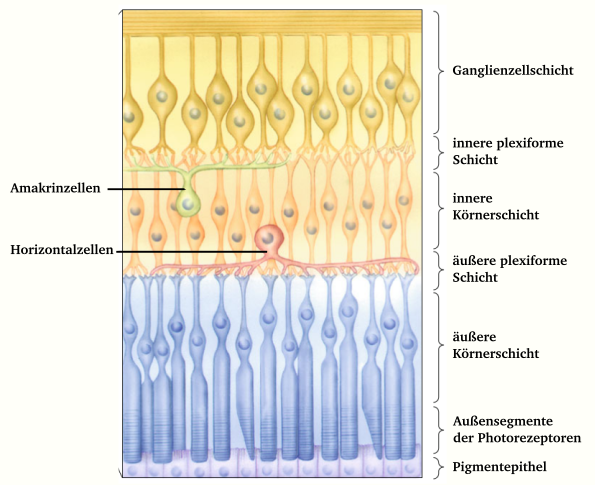
\includegraphics[width = 0.8\textwidth]{pictures/visual/retina.png}
    \caption[Schichten in der Retina]{\textbf{Schichten in der Retina.} Das Licht geht von oben durch die einzelnen Schichten, bis es von den Photopigmenten der Photorezeptoren absorbiert wird. \\
    Abbildung nach \textit{Neurowissenschaften}, Bear et al. \textsuperscript{\cite[Kap.~10]{neurowissenschaften_baer}}.}
    \label{fig:retina}
\end{figure}

\noindent Die Photorezeptoren werden in \textbf{Stäbchen} \index{Stäbchen} und \textbf{Zäpfchen} \index{Zäpfchen} unterschieden. Die Stäbchen ermöglichen, aufgrund ihrer hohen Sensitivität, ein Hell-Dunkel-Sehen. Bei den Zäpfchen unterscheidet man zwischen den blau-sensitiven, grün-sensitiven und rot-sensitiven Zäpfchen. Die Unterscheidung erfolgt anhand des Absorptionsspektrums der einzelnen Zäpfchen. Die Verteilung der Stäbchen und Zäpfchens über die Retina ist nicht konstant. Im Randbereich der Retina sind mehr Stäbchen vorhanden, während es zur \textbf{Fovea} \index{Fovea} hin weniger werden. Die Fovea selbst ist der Bereich der Retina, in dem es keine Stäbchen gibt, sondern nur Zäpfchen. Außerdem sind im Bereich der Fovea auch die anderen Zellschichten zur Seite verdrängt. Sie ist der Bereich des schärfsten Sehens \textsuperscript{\cite[Kap.~10]{neurowissenschaften_baer}}.

\subsubsection*{Das Optische Chiasma und der Optische Trakt}

Der linke und rechte Sehnerv ziehen über den optischen Kanal in die Schädelhöhle. An der Basis des Gehirns, unterhalb des \textit{Tuber cinereum} des Hypothalamus, laufen die beiden Sehnerven zum \textbf{Chiasma opticum} \index{Chiasma opticum} zusammen. 
Im Chiasma opticum kreuzen die Nerven aus dem nasalen Bereich des Gesichtsfelds auf die jeweils andere Seite. Im Chiasma opticum (Abb.~\ref{fig:optic_tract}~A) findet keine Verschaltung statt. Die Nervenbahnen kreuzen nur auf die andere Seite.
Da beim Menschen nur ein Teil der Nerven auf die andere Seite kreuzt, wird diese Kreuzung \textbf{Semidekussation} \index{Semidekussation} genannt \textsuperscript{\cite[Kap.~15]{crossman2014neuroanatomy}}. 

In Abbildung~\ref{fig:sehbahn_baer} ist die Sehbahn des Menschen abgebildet. Aufgrund der frontalen Augen des Menschen überlappen die beiden Sehfelder stark. Da Ratten lateral liegende Augen besitzen, ist bei ihnen eine bessere Rundumsicht möglich, jedoch ist das binokulare Gesichtsfeld kleiner (40~-~60\% Überlappung) \textsuperscript{\cite[Kap.~30]{paxinos2014rat}}.
Alles was auf der linken Gesichtsfeldhälfte abgebildet wird, wird auf der rechten Retinahälfte abgebildet und umgekehrt. Der linke und rechte Sehnerv, tragen jeweils die Informationen des gesamten Sehfeldes eines Auges bis zum Chiasma opticum. Dort kreuzen die Nerven aus dem nasalen Bereich der Retina auf die andere Seite. Danach verlaufen der linke und rechte Tractus opticus, \index{Tractus! opticus} diese tragen dann nur noch die Informationen aus einer Gesichtsfeldhälfte (rechter Tractus - linke Gesichtsfeldhälfte und umgekehrt), bis ins Gehirn \textsuperscript{\cite[Kap.~15]{crossman2014neuroanatomy}}.

\begin{figure}[H]
    \centering
    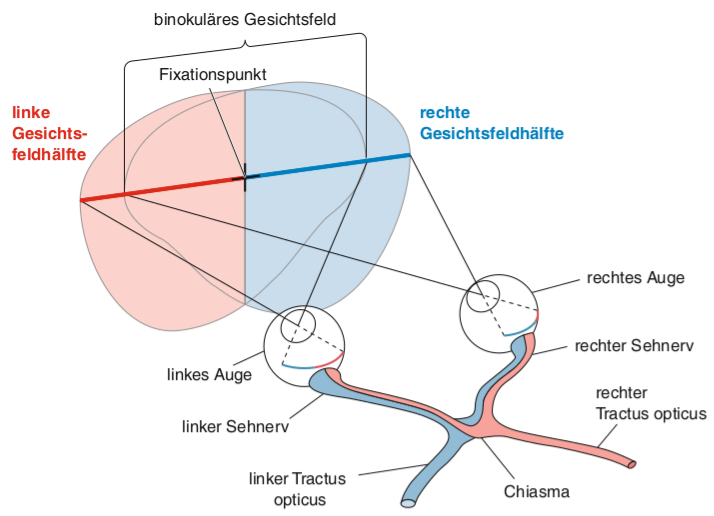
\includegraphics[width = 0.9\textwidth]{pictures/visual/Sehbahn.png}
    \caption[Die Sehbahn]{\textbf{Die Sehbahn.} Die Sehbahn des Menschen mit dem Verlauf der Nervenbahnen und der Projektionsbahnen der linken und rechten Gesichtsfeldhälfte.\\
    Abbildung nach \textit{Neurowissenschaften}, Bear et al. \textsuperscript{\cite[Kap.~10]{neurowissenschaften_baer}}.}
    \label{fig:sehbahn_baer}
\end{figure}

Der optische Trakt verläuft auf beiden Hemisphären um den \textit{Pedunculus cerebri} herum bis in den Nucleus geniculatum lateralis im Thalamus (Abb.~\ref{fig:optic_tract}~B~-~E). \textsuperscript{\cite[Kap.~15]{crossman2014neuroanatomy}}

\begin{figure}[H]
    \centering
    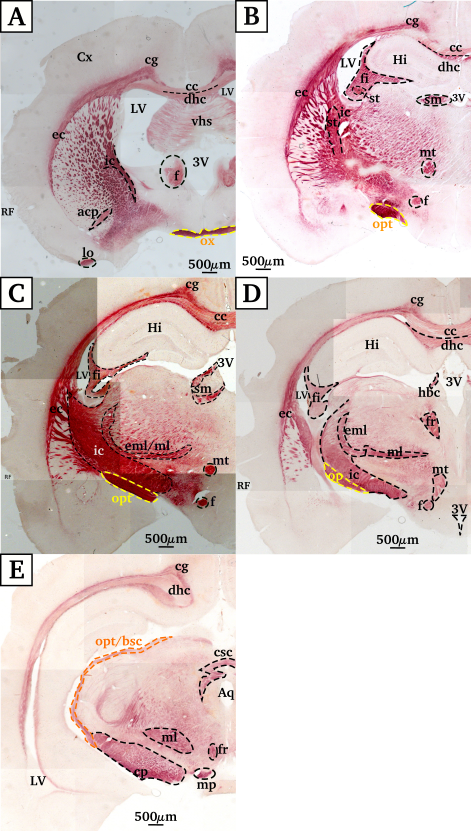
\includegraphics{pictures/visual/optic_tract.png}
    \caption[Das Optische Chiasma und der Optische Trakt]{\textbf{Das Optische Chiasma und der Optische Trakt.} Der Verlauf des optischen Trakts vom optischen Chiasma bis zum Thalamus. \textbf{A:}~F18-3, \textbf{B:}~F20-3, \textbf{C:}~F21-3, \textbf{D:}~F23-3, \textbf{E:}~F26-2.}
    \label{fig:optic_tract}
\end{figure}

\subsubsection*{Beschriftung und Kürzel}

\begin{table}[H]
\begin{tabular}{llcll}
           & 3V  & -          & dritter Ventrikel                                                       & \multicolumn{1}{c}{\textbf{}} \\
\textbf{A} & acp & -          & Commissura anterior, posteriorer Teil                                   & \multicolumn{1}{c}{}          \\
\textbf{}  & Aq  & -          & Aquädukt, Aqueductus mesencephali, Aquaeductus cerebri                  & \multicolumn{1}{c}{}          \\
\textbf{B} & bsc & -          & Brachium colliculi superioris                                           & \multicolumn{1}{c}{}          \\
\textbf{C} & cc  & -          & Corpus callosum                                                         & \multicolumn{1}{c}{\textbf{}} \\
\textbf{}  & cg  & -          & Cingulum                                                                & \multicolumn{1}{c}{\textbf{}} \\
\textbf{ } & cp  & -          & Pedunculus cerebri, Kleinhirn-Pedunkel                                  & \multicolumn{1}{c}{\textbf{}} \\
\textbf{ } & csc & -          & Commissura colliculi superioris                                         & \multicolumn{1}{c}{\textbf{}} \\
\textbf{}  & Cx  & -          & Cortex                                                                  & \multicolumn{1}{c}{}          \\
\textbf{D} & dhc & -          & dorsale Hippocampus-Kommissur                                           & \multicolumn{1}{c}{}          \\
\textbf{E} & ec  & -          & Capsula externa                                                         &                               \\
\textbf{ } & eml & -          & Lamina medullaris lateralis, external medullary lamina                  &                               \\
\textbf{F} & f   & -          & Fornix                                                                  &                               \\
\textbf{}  & fi  & -          & Fimbria                                                                 &                               \\
\textbf{}  & fr  & -          & Fasciculus retroflexus                                                  &                               \\
\textbf{H} & hbc & -          & Commissura habenularum                                                  &                               \\
\textbf{}  & Hi  & -          & Hippocampus                                                             &                               \\
\textbf{I} & ic  & -          & Capsula interna                                                         &                               \\
\textbf{L} & lo  & -          & lateraler olfaktorischer Tract, tractus olfactorius lateralis           &                               \\
\textbf{}  & LV  & -          & lateraler Ventrikel                                                     &                               \\
\textbf{M} & ml  & -          & medialer Lemniscus                                                      &                               \\
\textbf{}  & mp  & -          & Mammillar-Pedunkel                                                       &                               \\
\textbf{}  & mt  & -          & mammilothalamischer Trakt                                               &                               \\
\textbf{O} & opt & -          & optischer Trakt, Tractus opticus                                        &                               \\
\textbf{}  & ox  & -          & Chiasma opticum                                                         &                               \\
\textbf{R} & RF  & -          & Fissura rhinalis                                                        &                               \\
\textbf{S} & sm  & -          & Stria medullaris thalami                                                &                               \\
\textbf{}  & st  & -          & Stria terminalis                                                        &                               \\
\end{tabular}
\end{table}

\newpage
\subsubsection*{Der Corpus geniculatum laterale}

Der \textbf{Corpus geniculatum laterale} (\textbf{LGN}) \index{Corpus! geniculatum laterale} liegt im posterioren Teil des Thalamus und gehört zu den Nuclei des Kniehöckers (Abb.~\ref{fig:LGN}) \textsuperscript{\cite[Kap.~12]{crossman2014neuroanatomy}}. Im LGN terminieren die Ganglienzellen der ipsilateralen Gesichtshälfte, und bei frontalen Augen auch von die der contralateralen Netzhauthälften beider Retinae. Die Informationen aus den Ganglionzellen werden im LGN unter Einflussnahme des visuellen Cortex verarbeitet
\textsuperscript{\cite[Kap.~8.1]{trepel2011neuroanatomie}}.

\begin{figure}[H]
    \centering
    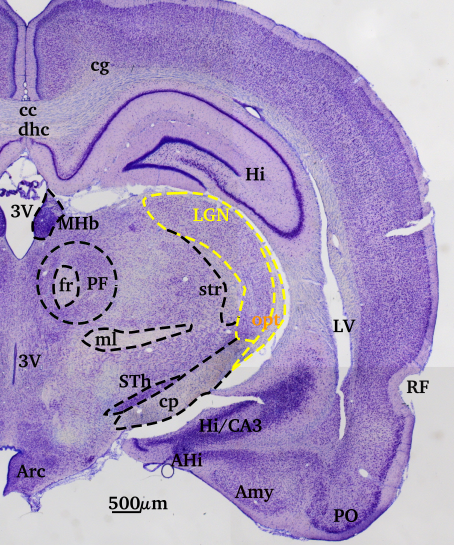
\includegraphics{pictures/visual/LGN.png}
    \caption[Corpus geniculatum laterale]{\textbf{Corpus geniculatum laterale.} Nissl-Färbung (N20-4) auf der Höhe des Diencephalons und des Cortex. Der Corpus geniculatum laterale (LGN) befindet sich auf der lateralen Seite im Thalamus. Die eingehenden Informationen kommen aus dem optischen Trakt (opt) der lateral, am Pedunculus cerebri (cp, Kleinhirn-Pedunkel) vorbei, in den LGN zieht. Im Schnitt auf derselben Höhe liegen prominente Strukturen, wie Teile des Hippocampus (Hi) und der (mediale) Nucleus habenulares (MHb). Des Weiteren sind in diesem Schnitt folgende Strukturen zu sehen: 
    dritter Ventrikel (3V), amygdaloid-hippocampaler Bereich (AHi), Amygdala (Amy), Nucleus arcuatus hypothalami (Arc), Ammon's Horn (CA3), Corpus callosum (cc), Cingulum (cg), dorsale Hippocampus-Kommissur (dhc), Fasciculus retroflexus (fr), lateraler Ventrikel (LV), medialer Lemniscus (ml), Nucleus parafascicularis (PF),  primärer  olfaktorischer  Cortex (PO), Fissura rhinalis (RF), Nucleus subthalamicus (STh), Radiatio thalami superior (str).}
    \label{fig:LGN}
\end{figure}

Der LGN ist bei Altweltaffen und dem Menschen aus sechs Schichten aufgebaut. 
In Abbildung~\ref{fig:schichtung-LGN} sieht man die sechs Schichten, die wie Hüte gestapelt den Corpus geniculatum laterale bilden. In Schicht~1 und~2 terminieren die M-Ganglienzellen, wobei in Schicht~1 die contralateralen Neurone terminieren und in Schicht~2 die der ipsilateralen Seite. Sie geben die Informationen an die \textbf{magnozellulären} LGN-Zellen weiter. Die Axone der P-Ganglienzellen terminieren in Schicht~3 bis~6 an den \textbf{parvozellulären} LGN-Zellen. Auch hier ist der Input aus den Augen streng getrennt. Es ergibt sich folgende Reihenfolge: Schicht~3: ipsilateral, Schicht~4: contralateral, Schicht~5: ipsilateral, Schicht~6: contralateral.
Zwischen den Schichten liegen die Schichten der \textbf{konizellulären} LGN-Zellen. Sie bekommen Input aus den nonM-nonP-Ganglienzellen \textsuperscript{\cite[Kap.~9.7]{heldmaier2003tierphysiologie}}.

\begin{figure}[H]
    \centering
    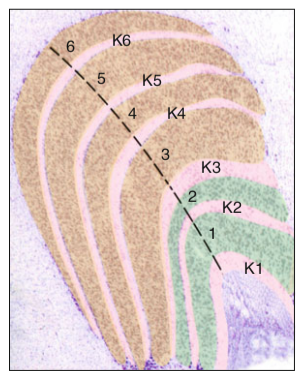
\includegraphics{pictures/visual/LGN_baer.png}
    \caption[Schichtung des LGN]{\textbf{Schichtung des LGN.} Die sechs Schichten des Corpus geniculatum laterale des Menschen. Schicht~1 und~2 bekommen Input aus den M-Ganglienzellen, Schicht~3 bis~6 aus den P-Ganglionzellen und die Schichten dazwischen aus den nonM-nonP-Ganglienzellen. Die Zellen des LGN in den zwischen Schichten werden konikuläre Zellen (K1~-~K6) genannt. Abbildung nach \textit{Neurowissenschaften}, Bear et al. \textsuperscript{\cite[Kap.~10]{neurowissenschaften_baer}}.}
    \label{fig:schichtung-LGN}
\end{figure} 

Aufgrund der Funktion der M-Ganglienzellen, die nicht zwischen Licht unterschiedlicher Wellenlänge unterscheiden, haben die magnozellulären LGN-Neurone ebenfalls farbenblinde rezeptive Felder. Sie reagieren vor allem auf Bewegungs-Stimmuli im rezeptiven Feld. In den Schichten~3 bis~6 bekommen die parvozellulären LGN-Neurone eingehende Informationen aus den farbsensitiven P-Ganglienzellen. Die rezeptiven Felder der LGN-Neurone in Schicht~3 und~4 sind blau/gelbe OFF~-~ON Felder, während die Neurone in Schicht~5 und~6 rot/grüne ON~-~OFF Felder sind \textsuperscript{\cite[Kap.~18]{smith2008biology}}.

Die Neurone des Corpus geniculatum laterale ziehen über die Seilstrahlung (\textbf{Radiatio optica}) \index{Radiatio optica} in den visuellen Cortex \textsuperscript{\cite[Kap.~8.1]{trepel2011neuroanatomie}}.


\subsubsection*{Der visuelle Cortex}

Der visuelle Cortex umfasst den primären und sekundären visuellen Cortex, sowie übergeordnete visuelle Cortexareale. Der visuelle Cortex liegt im Okzipitallappen im caudalen Bereich des Großhirns. 


\subsubsection*{Der primäre visuelle Cortex}

Der \textbf{primäre visuelle Cortex} (\textbf{V1}) \index{Cortex! primär visuell} umfasst das Brodmann-Areal 17. Er liegt auf der medialen Oberfläche der jeweiligen Hemisphäre und umgibt den \textbf{Sulcus calcarinus}\index{Sulcus! calcarinus}, wie in Abbildung~\ref{fig:V1} zu sehen ist \textsuperscript{\cite[Kap.~10]{neurowissenschaften_baer}}.
Der primäre visuelle Cortex unterscheidet sich vom Rest des Neocortex durch seine makroskopisch sichtbaren Streifen. Diese entstehen, da der Cortex mit Streifen (\textbf{Gennari-Streifen}) myelinisierter Fasern, die parallel zur Oberfläche in Schicht~4 verlaufen, durchzogen ist. Aus diesem Grund nennt man diesen Bereich des Cortex auch \textbf{Area striata} \textsuperscript{\cite[Kap.~18]{smith2008biology}}.

Die Fasern aus dem LGN ziehen in den ipsilateralen primären visuellen Cortex und terminieren dort in Schicht~4. Die eingehenden Informationen sind in dieser Schicht streng monokular getrennt. Die binokulare Verarbeitung findet in den anderen Schichten (II-VI) statt. Eine Hemisphäre in V1 verarbeitet etwas mehr als die Hälfte des Sehfeldes. Die Sehfelder überlappen an der vertikalen Mittellinie \textsuperscript{\cite[Kap.~25]{kandel2013principles}}.
Wie in Abbildung~\ref{fig:V1} zu sehen ist, entspricht die Größe der Repräsentation der einzelnen Bereichen des Sehfeldes im Cortex nicht der Größe des zugehörigen Bildes auf der Retina. Die Bereiche der Fovea und um die Fovea herum nehmen mehr cortikale Fläche ein als die Randbreiche der Retina. Die cortikale Flächengröße, die Input aus einem Sehbereich von einem Grad bekommt, wird durch den \textbf{Magnifikationsfaktor} berechnet und nimmt zur Fovea hin ab \textsuperscript{\cite[Kap.~25]{kandel2013principles}}.
\\
\\
\noindent Wie bereits erwähnt, verarbeiten die anderen Schichten im primären visuellen Cortex die Informationen aus beiden Augen. Der Aufbau dieser Schichten ist aber weiterhin sehr geordnet. Man unterscheidet in Schichten im generellen zwischen Blobs und Interblobs.

Die rezeptiven Felder in den Interblobs sind nicht mehr rund, wie in den vorherigen Verarbeitungszentren, sondern rechteckig. Die rezeptiven Felder verarbeiten Balkenstimuli gewisser Orientierung im rezeptiven Feld oder reagieren auf nur eine bestimmte Bewegungsrichtung eines Balkens. Die rezeptiven Felder reagieren in V1 nur noch selten auf stationäre Stimuli und häufiger auf Bewegung im rezeptiven Feld. \textsuperscript{\cite[Kap.~18]{smith2008biology}}

Rezeptive Felder mit einer bestimmten Richtung befinden sich in einer Reihe im Cortex. Diese bilden dann sogenannte Orientierungssäulen. Orthogonal dazu verlaufen in Schicht~4 die okulären Dominanzsäulen in den jeweils nur die rezeptiven Felder eines Auges liegen \textsuperscript{\cite[Kap.~10]{neurowissenschaften_baer}}.
In den Schichten~2 und~3 verlaufen auch noch sogenannte Cytochromoxidase-Blobs. In diesen liegen konzentrische rezeptive Felder, die auf Farbstimuli reagieren \textsuperscript{\cite[Kap.~18]{smith2008biology}}.\\

\noindent Vom primären visuellen Cortex aus projizieren die Neurone in den sekundären visuellen Cortex der in der sogenannten Area extrastriata liegt. 


\begin{figure}[H]
    \centering
    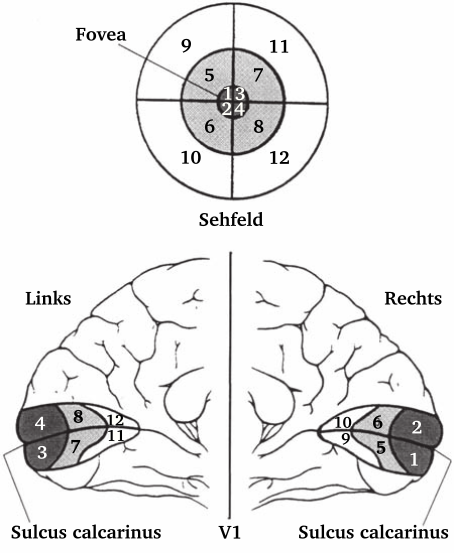
\includegraphics[width = 0.6\textwidth]{pictures/visual/V1.png}
    \caption[Der primäre visuelle Cortex]{\textbf{Der primäre visuelle Cortex.} Die Abbildung des Sehfeldes auf dem primären visuellen Cortex. Das Sehfeld kann in vier Quadranten eingeteilt werden. Der erste und zweite Quadrant (linkes Sehfeld) werden auf der rechten Hemisphäre abgebildet. Der dritte und vierte Quadrant werden auf der linken Hemisphäre abgebildet. Die Sehbereiche der Fovea (1~-~4) werden im caudalen Bereich von V1 abgebildet, wohingegen die Sehfelder distal zur Fovea (9~-~12) im rostralen Bereich abgebildet werden.\\
    Abbildung nach \textit{Biology of Sensory Systems}, Smith \textsuperscript{\cite[Kap.~18]{smith2008biology}}.}
    \label{fig:V1}
\end{figure}


\subsubsection*{Höhere visuelle Verarbeitungszentren und coritco-cortikale Verbindungen}

Die \textbf{Area extrastriata} ist das Gebiet, welches die höheren visuellen Verarbeitungszentren umfasst. Diese sind, wie auch der primäre visuelle Cortex, in Karten des Sehfeldes aufgebaut. Die neuronale Repräsentation der visuellen Welt als Bild ihrer Selbst, nennt sich \textbf{Retinotopie}. \index{Retinotopie} Die Verschaltung der verschiedenen visuellen Areale ist ein komplexes System, das bis heute noch erforscht wird. Zwei große Informationsverarbeitungswege verarbeiten die Informationen aus dem visuellen System. Es wird zwischen dem \textbf{ventralen Pfad} und dem \textbf{dorsalen Pfad} unterschieden \textsuperscript{\cite[Kap.~25]{kandel2013principles}}.
\\
\\ \noindent Der \textbf{ventrale Pfad} zieht sich über V4 in den Temporallappen (Abb.~\ref{fig:visual_pathway_cortex}). Im Großen und Ganzen werden im ventralen Pfad Informationen über das Objekt selbst verarbeitet. Er ist an der bewussten Wahrnehmung der visuellen Welt und der Wiedererkennung von Objekten beteiligt. Die meisten eingehenden Informationen bekommt der ventrale Pfad aus den Blobs und den Interblobs, die ihre Informationen wiederum von parvozellulären LGN-Neuronen erhalten. Er erhält trotzdem auch Informationen aus dem magnozellularen und dem konikularen System \textsuperscript{\cite[Kap.~10]{neurowissenschaften_baer}}.


Der \textbf{dorsale Pfad} zieht über das Medio-Temporalareal (MT) weiter in den  Parietallappen (Abb.~\ref{fig:visual_pathway_cortex}). Ihm wird die Analyse von Bewegungen, die visuelle Kontrolle von Handlungen  
und die räumlichen Organisation von Objekten zugeschrieben. Die meisten eingehenden Informationen bekommt der dorsale Pfad aus den magnozellulären Neuronen in V1. Auch der dorsale Pfad erhält zudem Informationen aus den anderen Systemen \textsuperscript{\cite[Kap.~10]{neurowissenschaften_baer}}.

\begin{figure}[H]
    \centering
    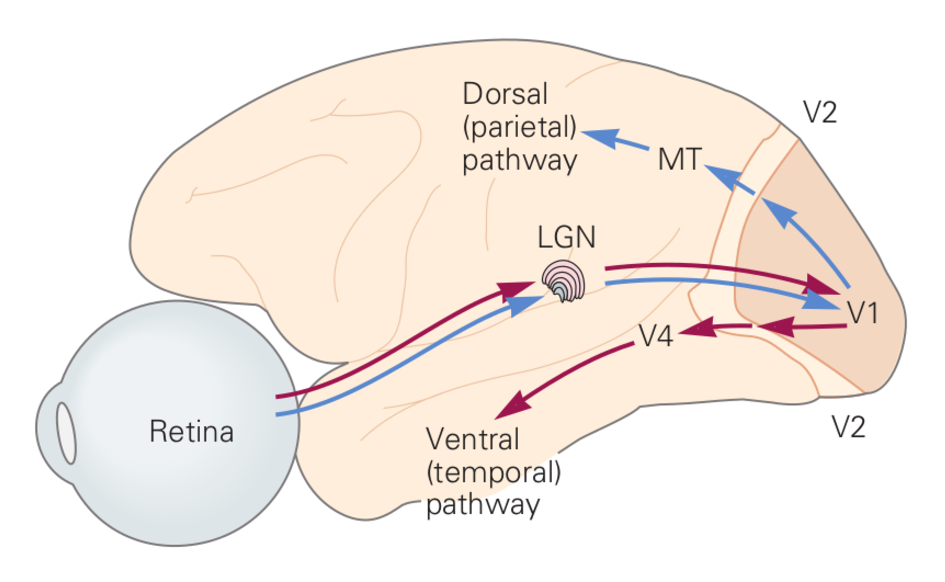
\includegraphics{pictures/visual/visual_Cortex.pdf}
    \caption[Visuelle Verarbeitungszentren im Cortex]{\textbf{Visuelle Verarbeitungszentren im Cortex.} V4: vierter visueller Cortex, MT: Medio-Temporallappen.\\
    Abbildung nach \textit{Principles of Neural Science}, Kandel et al. \textsuperscript{\cite[Kap.~27]{kandel2013principles}}.}
    \label{fig:visual_pathway_cortex}
\end{figure}


